\documentclass[a4paper, 12pt]{book}

% Paquetes básicos de LATEX
\usepackage{amsmath, amssymb}
\usepackage[T1]{fontenc}
\usepackage[utf8]{inputenc}
\usepackage[spanish]{babel}

% Título y autor
\title{Título del proyecto}
\author{Daniel Gómez}

% Para cambiar márgenes
\usepackage[a4paper]{geometry}
\geometry{left=3cm, right=3cm}

% Para quitar encabezado, pie de página y numeración en páginas vacías
\usepackage{emptypage}

% Para añadir figuras y su path
\usepackage{graphicx}
\graphicspath{{figures/}}

% Para modificar encabezados y pie de página
\usepackage{fancyhdr}
\fancyhf{} % Limpia los encabezados y pie de página
\lhead[\leftmark]{Daniel G. R.}
\rhead[Daniel G. R.]{\rightmark}
\cfoot[\thepage]{\thepage}

% Añadir línea separatoria en el encabezado
\renewcommand{\headrulewidth}{0.4pt}

% Paquete para añadir enlaces entre referencias
\usepackage[hidelinks]{hyperref}

% Comando creado para añadir figuras más rápido y más limpio
\newcommand{\addimage}[4]{
\begin{figure}[h]
\begin{center} \label{fig:#2}
\includegraphics[width=#4\textwidth]{#1}
\end{center}
\caption{#3}
\end{figure}
}



% Paquete para bibliografías
\usepackage[
backend=biber,
style=numeric,
sorting=none,
dateabbrev=false,
citestyle=numeric
]{biblatex}

\addbibresource{bibliografia.bib}

\begin{document}

\pagestyle{fancy}

\maketitle

\tableofcontents

\part{Introducción}
\pagenumbering{arabic}

\chapter{Introducción y visión general}


En este capítulo se hará una breve introducción para entender el contexto de este trabajo y el porqué de la necesidad del mismo. Se comentará la importancia de la localización para los seres humanos y se hará una introducción sobre los mapas utilizados por los robots para localizarse. Finalmente se expondrá la estructura del documento.\\

\section{La localización como una necesidad}

Que levante la mano quien no se ha perdido alguna vez por los despachos de alguna de las facultades, sobre todo en esos ambientes prácticamente idénticos entre sí. Todo ser humano alguna vez se ha parado en seco, ha mirado a un lado y a otro con cara de desaprobación y se ha preguntado: \textit{¿dónde estoy?} Estas situaciones, a veces incómodas, se deben esencialmente a que todo ser vivo con capacidad para desplazarse por un entorno necesita localizarse y orientarse si quiere alcanzar un objetivo, más aún si dicho entorno es totalmente desconocido.\\

A lo largo de los años, los seres humanos hemos utilizado multitud de métodos para la orientación, incluso en las situaciones más desfavorables. Un estudio para la revista \textit{The Royal Society} de la Universidad de Rennes sostiene que los vikingos usaban una variedad de calcita para calcular dónde se encontraba el sol utilizando la polarización de la luz dispersada por las nubes. Esta piedra solar se llama ``Espato de Islandia'' y les permitía orientarse incluso en fechas donde el sol parecía no querer mostrarse, algo que sucede muy frecuentemente en los mares nórdicos \cite{vikingos}. Hoy en día, con el uso de la tecnología GPS y de aplicaciones que la implementan como Google Maps, hemos cambiado esa piedra solar por un dispositivo electrónico que, no solo nos localiza y orienta en prácticamente cualquier situación, sino que lo hace con un error casi despreciable. Pese al avance de las tecnología de localización como GPS, existen ciertas situaciones en las que es complicado aprovecharse de ellas, como por ejemplo en los entornos indoor. En estos caso, los satélites no son capaces de comunicarse con nuestros dispositivos, por lo que necesitamos otro mecanismo para localizarnos.\\

%\begin{figure}[H]
%	\begin{center} 
%	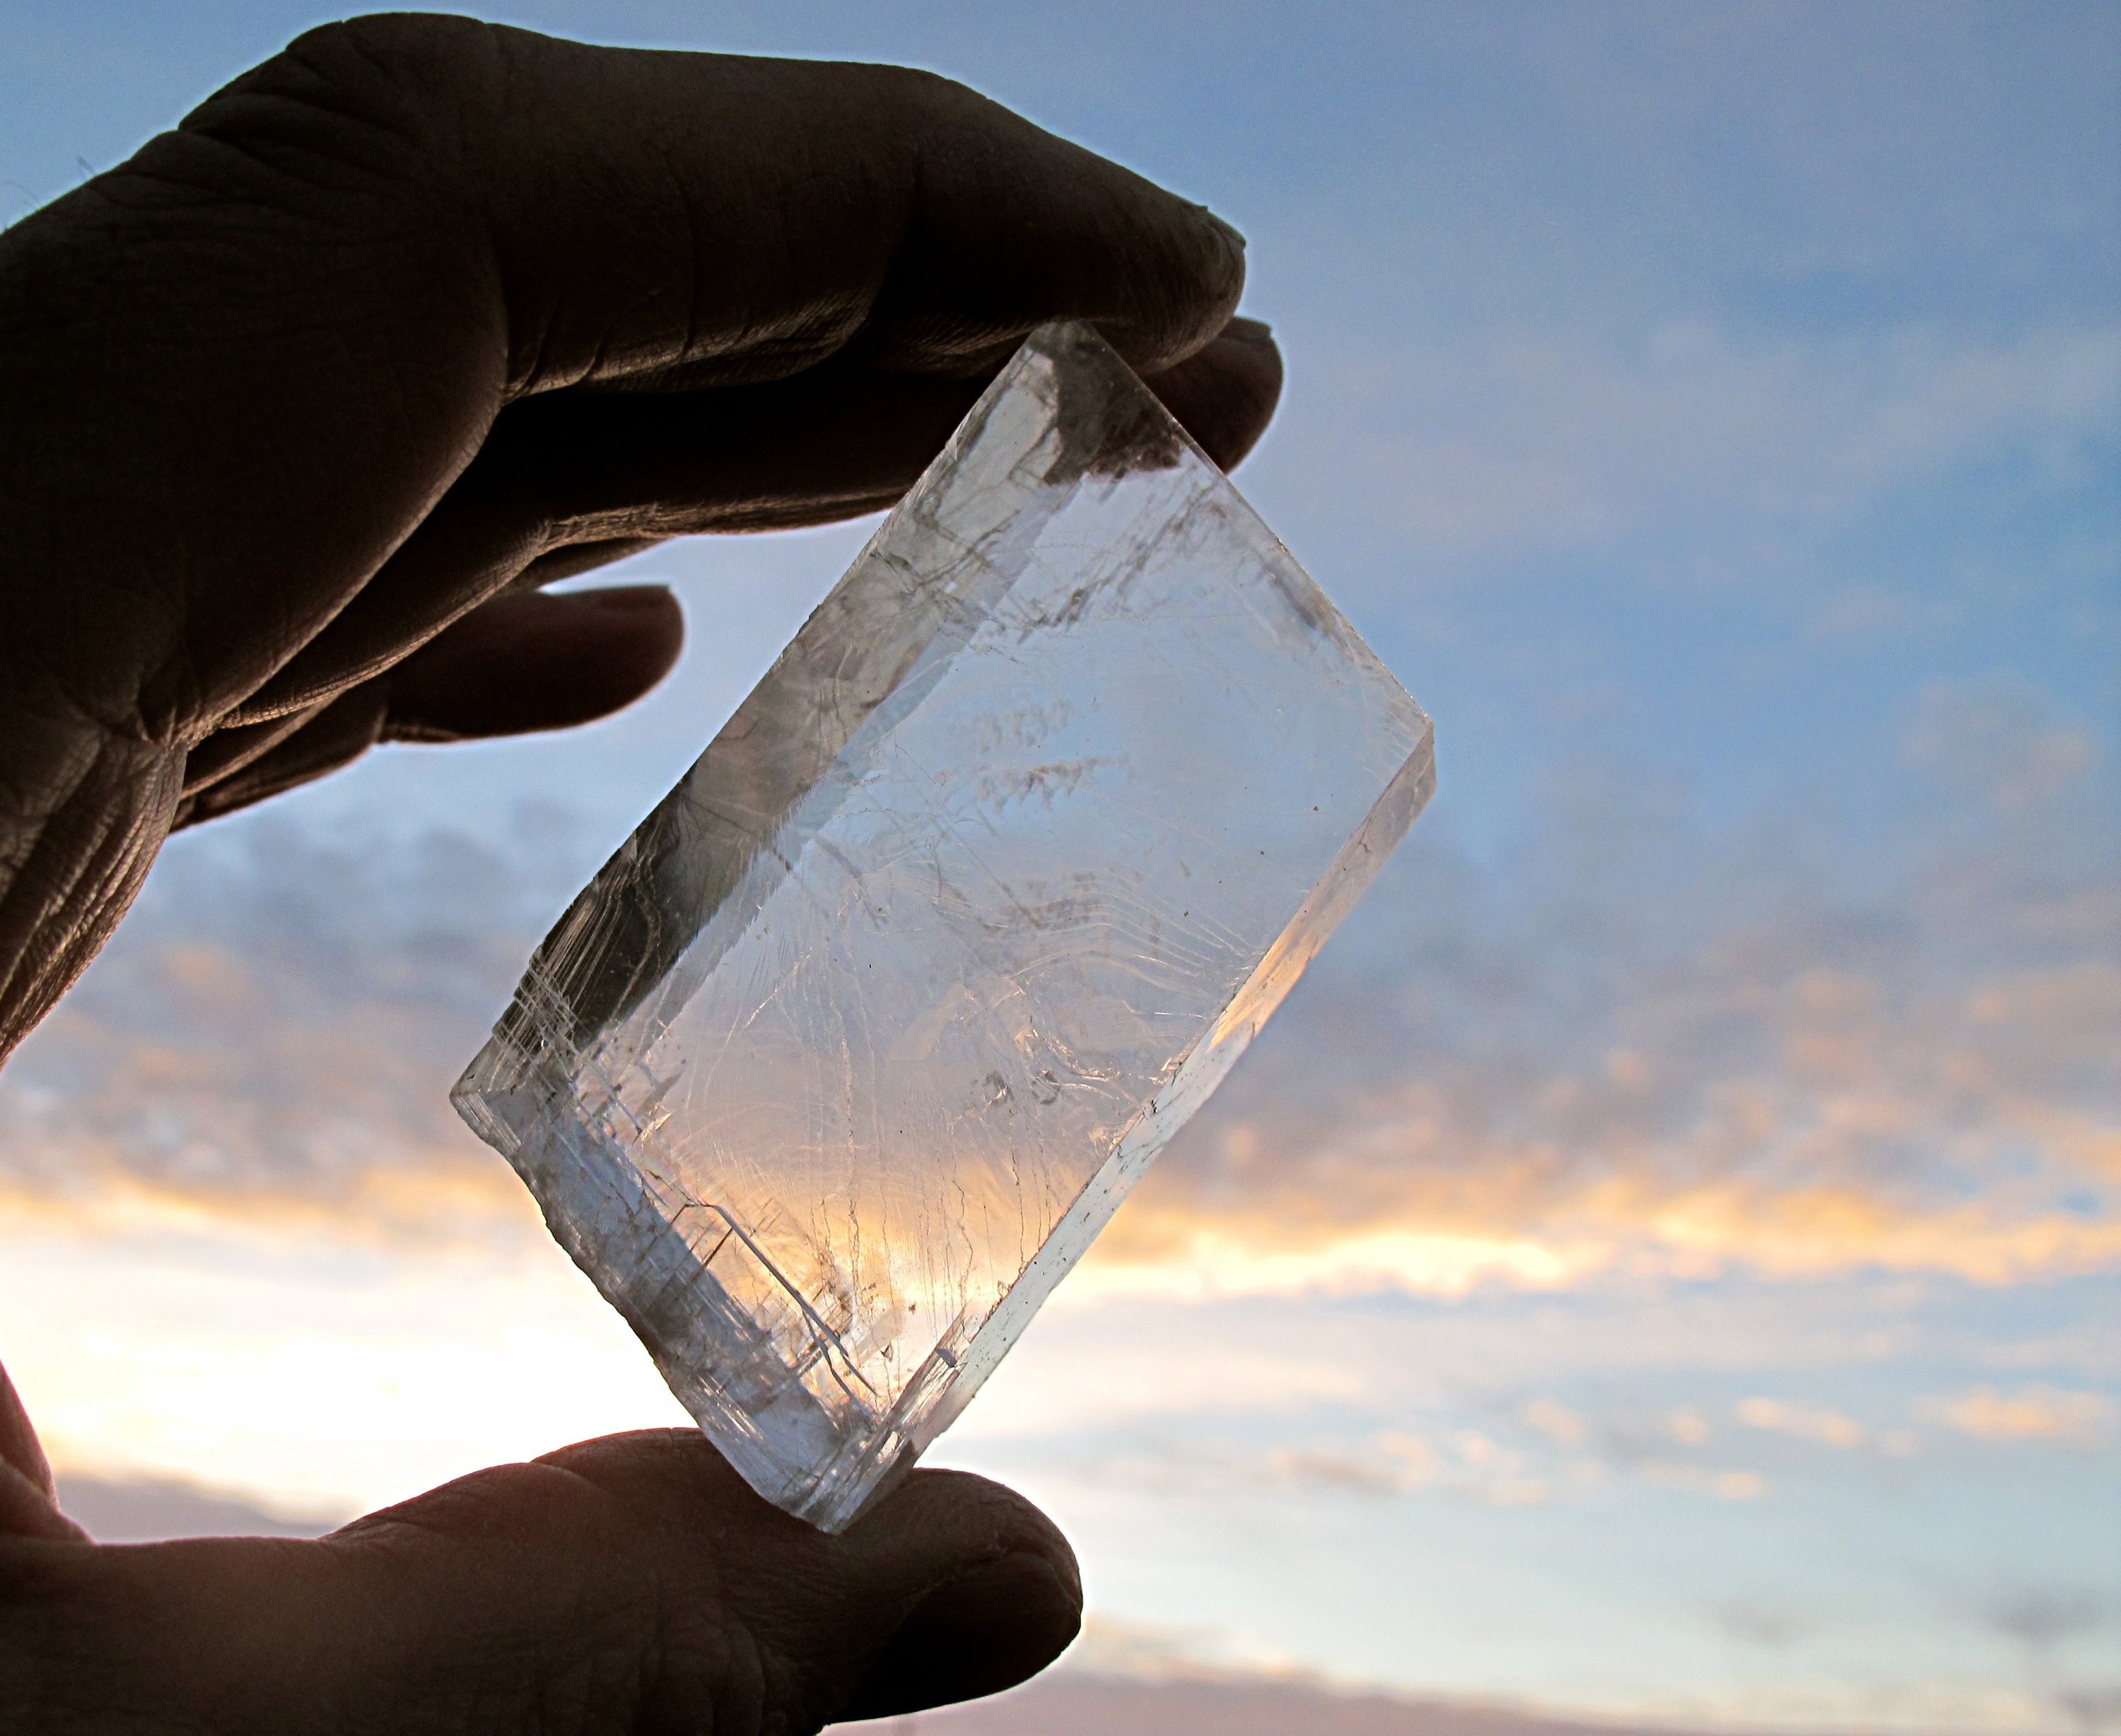
\includegraphics[width=0.5\textwidth]{espato_islandia.jpg}
%	\end{center}
%	\caption{Espato de Islandia. Variedad de piedra caliza \cite{espato}}
%	\label{fig:espato}
%\end{figure}

En la figura \ref{fig:metro} se muestra una parte del plano de la red de metro de la Comunidad de Madrid. A primera vista, uno se pierde entre tanto entresijo de líneas de colores pero si se establece una estación de origen y otra de destino, este plano facilita concretar el camino a tomar. Además, en las estaciones suele haber una gran cantidad de señalizaciones que hacen aún más fácil la localización. Entonces, si los humanos, seres inteligentes con percepción visual y capacidad de razonamiento, necesitamos localizarnos para alcanzar un objetivo, ¿porqué no lo iban a necesitar los robots? \\

\begin{figure}[h]
	\begin{center} 
	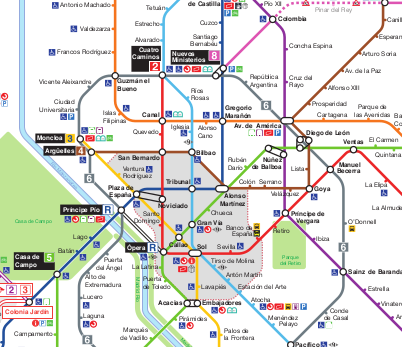
\includegraphics[width=0.4\textwidth]{plano_metro.png}
	\end{center}
	\caption{Detalle de la red de metro de la Comunidad de Madrid. \cite{metro_madrid}}
	\label{fig:metro}
\end{figure}

%\begin{figure}[H]
% \centering
%  \subfloat[Coeficiente $K=0$]{
%    \includegraphics[width=0.3\textwidth]{p6/simk0_ej1.png}}
%  \subfloat[Coeficiente $K=1$]{
%    \includegraphics[width=0.3\textwidth]{p6/simk1_ej1.png}}
% \caption{Simulación de la posición cartesiana para diferentes valores de %$K$}
% \label{fig:p6:sim_ej1}
%\end{figure}

La robótica móvil ha ido evolucionando a un ritmo vertiginoso desde que comenzó a desarrollarse. En los años sesenta se diseñó el apodado como \textit{SHAKEY} o ``el primer robot inteligente móvil del mundo'' según el IEEE (Instituto de Ingenieros Eléctricos y Electrónicos, del inglés \textit{Institute of Electrical and Electronics Engineers}). Este robot era el primero de su generación capaz de navegar en un entorno no controlado, sirviéndose de múltiples dispositivos que le proporcionaban información sobre la distribución de los elementos que le rodeaban, dándole la posibilidad al robot de evitarlos durante el trayecto \cite{shakey1}.\\

\begin{figure}[h]
	\begin{center} 
	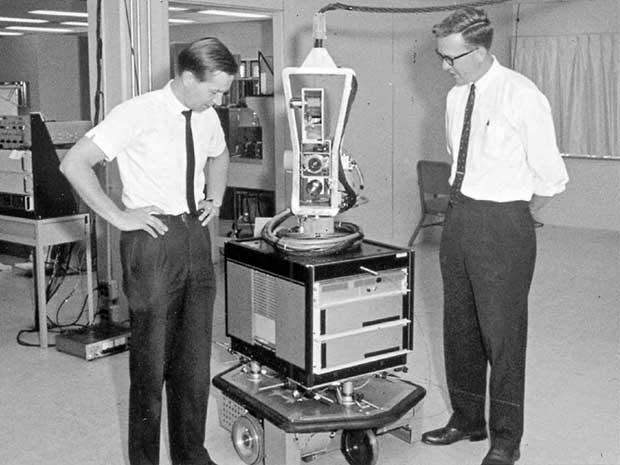
\includegraphics[width=0.8\textwidth]{shakey.jpg}
	\end{center}
	\caption{Foto tomada del robot SHAKEY en 1968. \cite{shakey2}}
	\label{fig:shakey}
\end{figure}


Un robot autónomo móvil (ARM) es un robot capaz de navegar a través de un entorno sin supervisión directa por parte de un operador humano ni la necesidad de disponer de un ruta fijada previamente. Para poder llevarlo a cabo, los robots disponen de multitud de sensores que les permiten percibir e interpretar el entorno, dotando al robot de la capacidad de navegar por el mismo evitando obstáculos, tanto fijos como móviles. Para poder realizar una navegación de alto nivel que les permita ir desde un punto origen a otro punto destino, los robots se sirven de mapas. Un mapa es una representación bidimensional del entorno. De forma general, podemos distinguir dos tipos de mapas de aplicación a la robótica: los mapas métricos y los mapas topológicos. Los mapas métricos (figura \ref{fig:mapas}, izquierda) dividen el entorno en una rejilla donde cada celda representa una probabilidad de estar ocupada o de no estarlo. Si se discretiza esa probabilidad el resultado es un mapa de ocupación, (también llamado \textit{floorplan} o ``plano de suelo'', en un ámbito menos técnico), si no, se obtiene un mapa probabilístico. El mapa métrico más simple es el formado por un conjunto de referencias visuales o \textit{landmarks} de posición conocida que ayudan al robot a estimar su posición. Los mapas topológicos (figura \ref{fig:mapas}, derecha) están basados en grafos y representan la conectividad entre cada uno de sus nodos. Existe una tercer tipo de mapa que es un híbrido entre los comentados y es el más utilizado para los robots: utilizan los grafos para la generación de trayectorias (navegación) y el mapa métrico para la localización.\\

\begin{figure}[H]
 \centering
  \subfloat[Ejemplo de mapa métrico: mapa de ocupación \cite{thrun}]{
    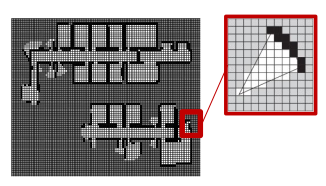
\includegraphics[width=0.35\textwidth]{mapa_ocupacion.png}}
  \hspace{2cm}
  \subfloat[Mapa topológico: líneas del metro de Málaga \cite{metro_malaga}]{
    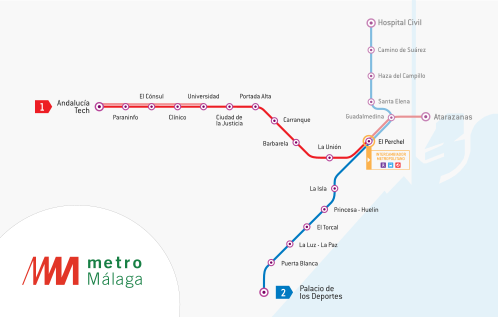
\includegraphics[width=0.3\textwidth]{metro_malaga.png}}
 \caption{Ejemplos de tipos de mapas.}
 \label{fig:mapas}
\end{figure}

Los mapas métricos más utilizados en la robótica móvil son los mapas de ocupación o \textit{floorplans}. Son generados en una primera fase de inspección del entorno, empleando los mismos sensores que luego servirán para la navegación autónoma. Tradicionalmente, estos mapas de ocupación son generados empleando un láser 2D o LIDAR (dado su gran alcance y amplio campo de visión), generando por tanto mapas bidimensionales que especifican aquellas zonas del entorno que están libres de obstáculos y por tanto susceptibles de navegación, y aquellas que no lo están. No obstante, dado que un láser 2D no puede distinguir entre los objetos detectados, los mapas de ocupación bidimensionales generados con este sensor contienen, no sólo los elementos estructurales del entorno como paredes, puertas, columnas, etc., si no que incluyen multitud de objetos como mesas y sillas, camas, cajas e incluso personas si estaban presentes en el momento de generar el mapa.\\

La inclusión de estos elementos no estructurales en el mapa de ocupación puede ocasionar problemas si se pretende utilizar ese mapa durante un largo período de tiempo. El mapa generado no estaría preparado si el entorno que representa sufre algún tipo de modificación de mobiliario, por lo que sería necesario volver a generar un nuevo mapa, con todo lo que eso conlleva. Sin ir más lejos, en la Escuela de Ingenierías Industriales hay muchos elementos que no pertenecen a la estructura del edificio que, si hoy mismo se utilizara un robot equipado con un láser 2D para generar un mapa, ocasionarían los problemas ya comentados. Estos elementos son, por ejemplo, las impresoras que hay en algunas zonas, las máquinas de refrescos y snacks, papeleras, carteles publicitarios, las nuevas mesas instaladas en la zona central, etc (figura \ref{fig:laser_vs_rgbd}). En la figura \ref{fig:laser_vs_rgbd} se muestra un ejemplo de lo que se quiere conseguir aprovechando las ventajas de los sensores RGBD frente a los láseres 2D aplicado a la Escuela de Ingenierías.\\

\begin{figure}[H]
	\begin{center} 
	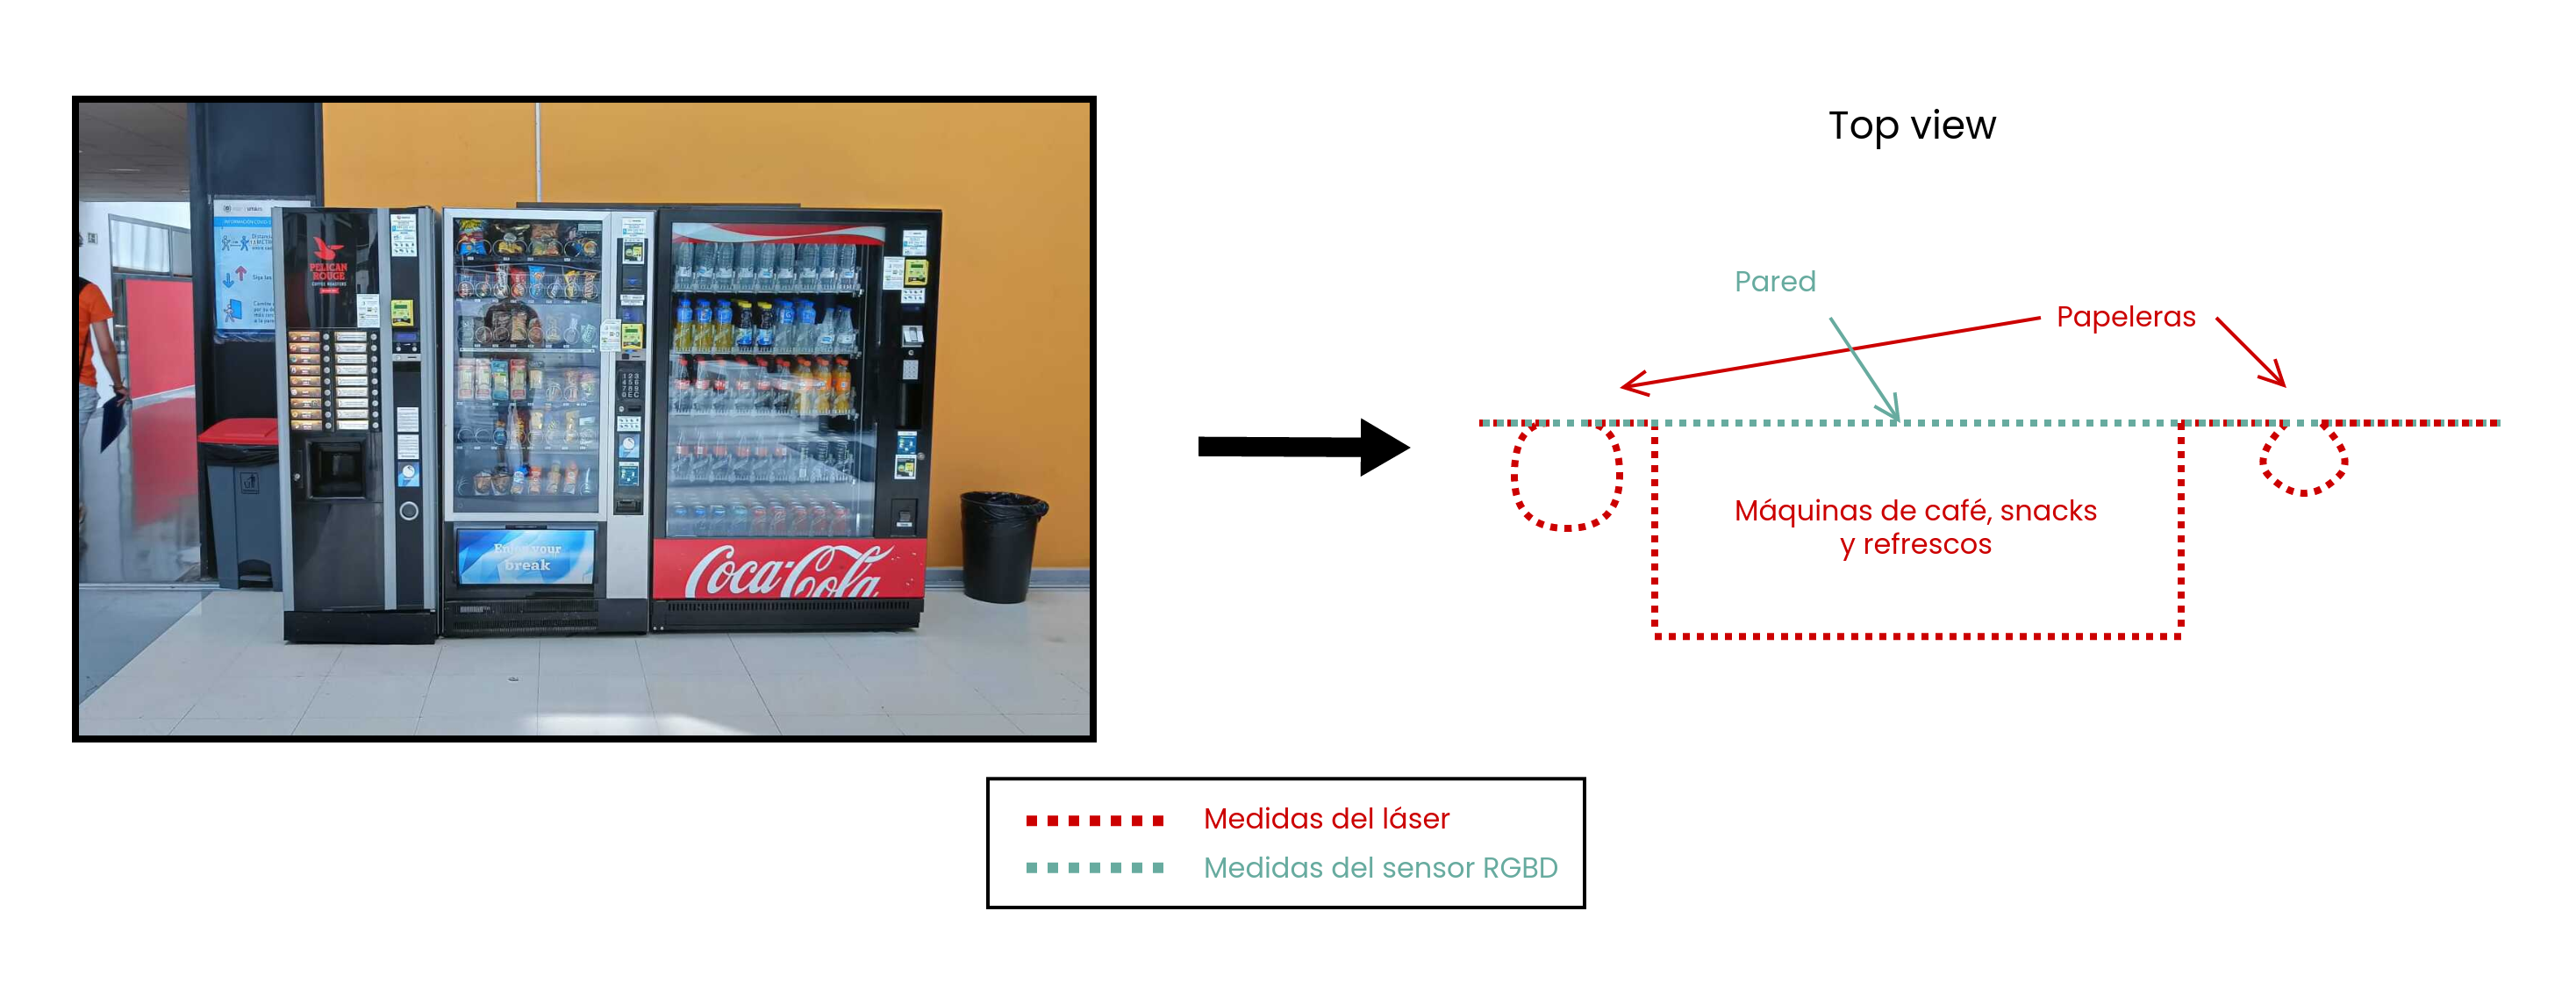
\includegraphics[width=\textwidth]{laser_vs_rgbd.png}
	\end{center}
	\caption{Comparación teórica del resultado de una medición de un láser 2D y un sensor RGBD sobre elementos presentes en la Escuela de Ingenierías Industriales.}
	\label{fig:laser_vs_rgbd}
\end{figure}

Otro ejemplo se puede ver en la figura \ref{fig:errores_laser} donde se muestra un mapa generado de un entorno virtual a través de un láser 2D de 360º. Como se puede observar hay zonas, marcadas con numeración, en las que el mapa no representa fielmente las dimensiones reales de la vivienda. De modo que, si los objetos que no forman parte de la estructura modifican su posición después de la primera fase de análisis, el mapa de ocupación generado no podría ser utilizado por el robot para la navegación. \\

\begin{figure}[h]
	\begin{center} 
	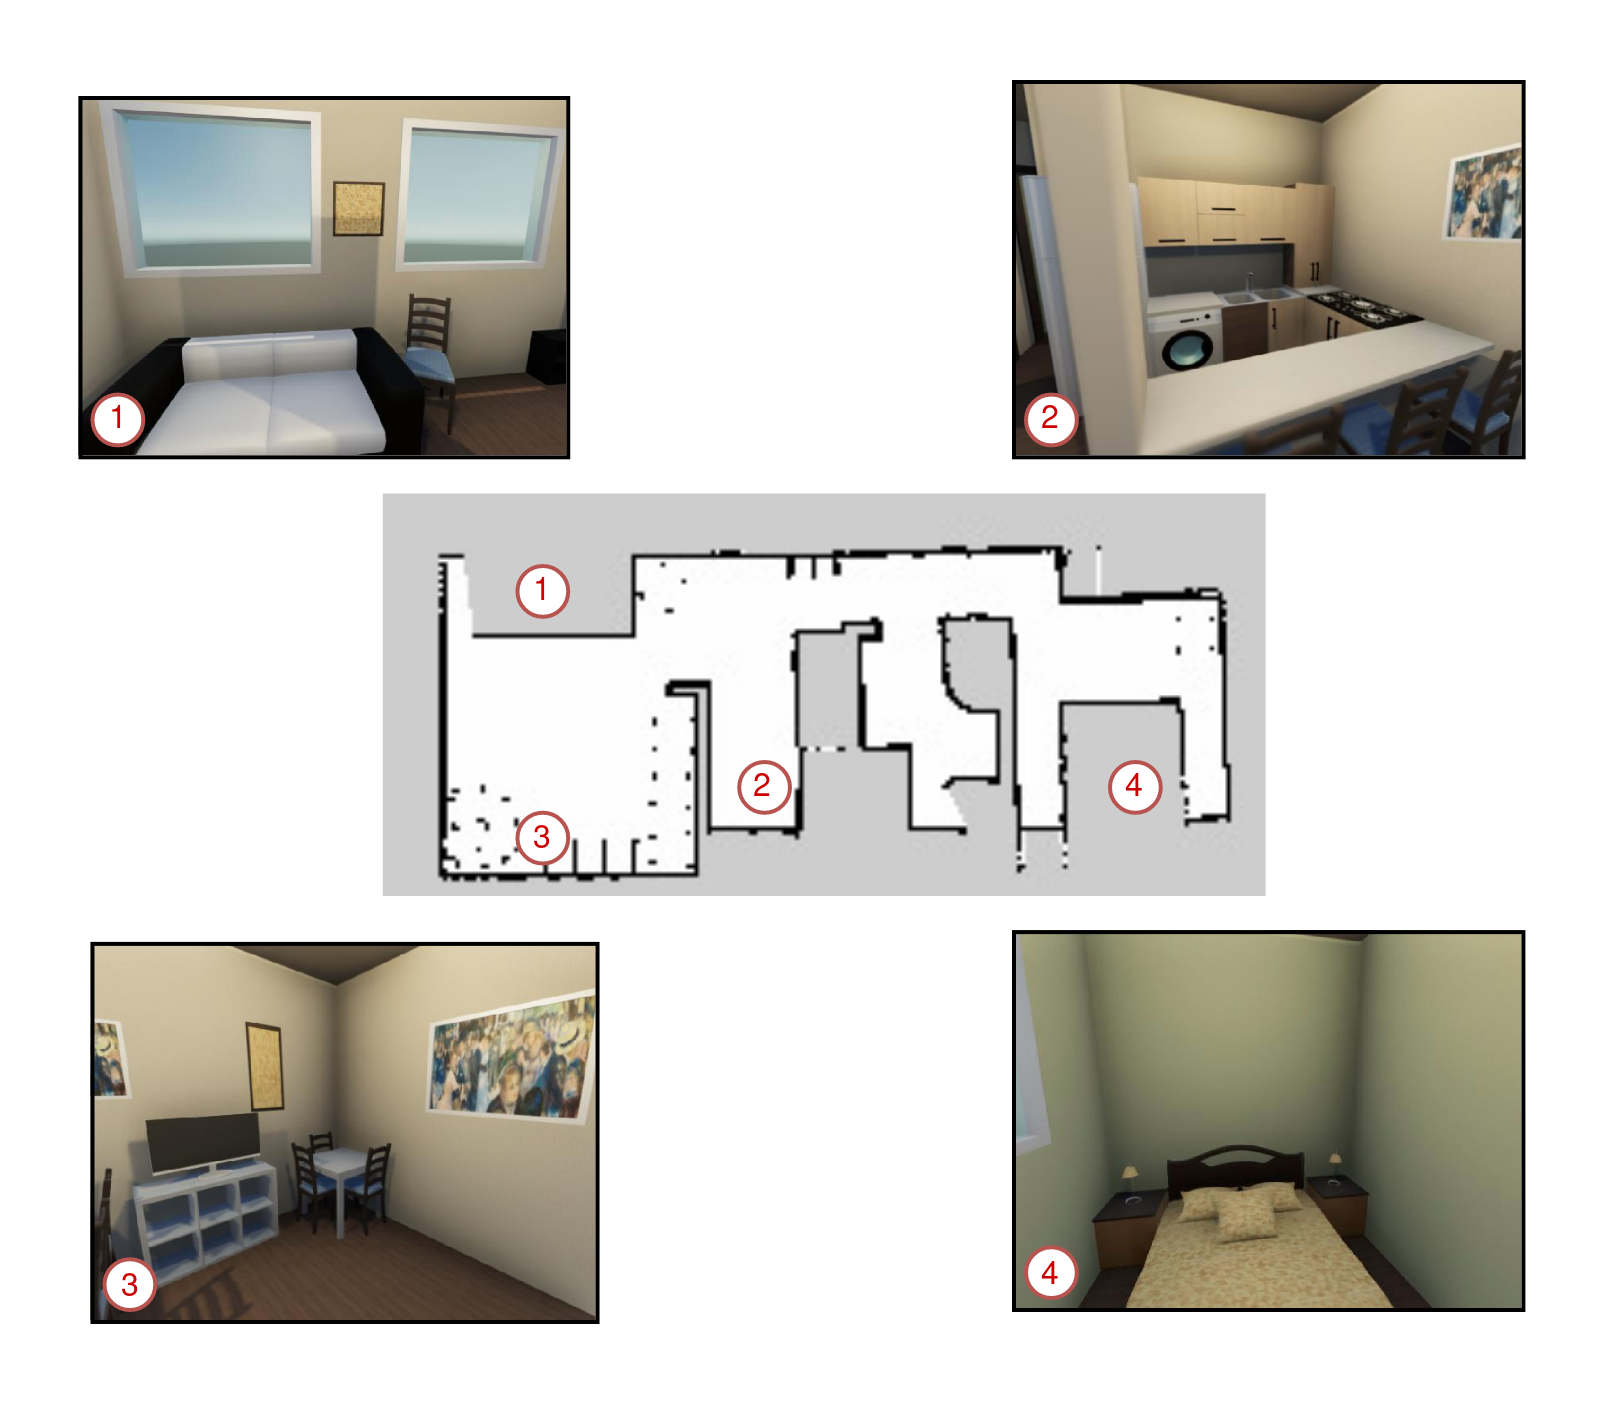
\includegraphics[width=0.6\textwidth]{IlustracionErroresMapa.png}
	\end{center}
	\caption{Mapa generado con el barrido de un láser. Las zonas enumeradas muestran que el mapa generado no representa fielmente la estructura del entorno debido a la presencia de elementos que pueden variar en su posición como un sofá, una silla, una cama, etc.}
	\label{fig:errores_laser}
\end{figure}

Dado que estos métodos de generación de mapas de ocupación mediante láser 2D sufren frente a la variabilidad en la distribución, surge la idea de utilizar otros sensores que permitan discernir entre los distintos elementos que pudieran formar parte del entorno. Los sensores RGBD son cámaras que, además de proporcionar información sobre el color, ofrecen la distancia a la que se encuentra cada píxel captado en la imagen con respecto a la cámara. Por lo tanto, ofrecen información en 3D del dominio, lo que abre más posibilidades a la hora de percibir e interpretar la información captada mediante los sensores. \\

En este proyecto se pretende analizar una posible solución al problema de fiabilidad en la representación de los mapas de ocupación realizados con sensores LIDAR mediante el uso de sensores RGBD para generar \textit{floorplans} fieles a la estructura invariable del entorno. Entre las utilidades de conseguir un mapa sin los objetos móviles, las más destacadas son:

\begin{itemize}

	\item La más importante es la posibilidad de tener un mapa que permita al robot localizarse aún con los cambios que puedan surgir a lo largo del tiempo en los elementos que conforman el entorno. Así se evita tener que generar un nuevo mapa cada vez que surja algún cambio significativo.
	\item En aplicaciones de realidad aumentada para el diseño de interiores, este sistema permitiría obtener las dimensiones reales de la vivienda y así tener una idea en primera persona del cambio de mobiliario o de una nueva organización del mismo.
	\item Normalmente existe una clara disparidad entre el plano de una vivienda o de un edificio diseñado por el arquitecto y el producto final. Con este mapa generado sería posible comparar y obtener un plano fiel a la realidad y así validar las dimensiones reales de la infraestructura.

\end{itemize}



\section{Objetivo}

Dado que los robots utilizan los mapas de ocupación o \textit{floorplans} para localizarse y navegar en un entorno, es necesario que éstos sean lo más fiel posible a la estructura real del edificio o de la vivienda. Esto resulta imposible si durante la fase de obtención del mapa existen elementos que no pertenecen a la infraestructura, ya que provocan que el mapa resultante no sea fiel a las dimensiones reales del entorno.\\

Debido a la necesidad y utilidad de obtener mapas de ocupación sin elementos cambiantes, el objetivo de este trabajo es utilizar la información proporcionada por sensores RGBD para la generación de \textit{floorplans}, solucionando problemas de variabilidad en el entorno que perjudican seriamente la fiabilidad del mapeado mediante sensores láser.\\

Se obtendrá información acerca de la profundidad de los píxeles captados y se escogerán aquellos puntos menos restrictivos (más alejados) para generar un láser artificial que permita la creación del mapa de ocupación mediante algoritmos de mapeado.\\

Paralelamente, se utilizará un modelo entrenado de inteligencia artifical, YOLO, para detectar los elementos de la imagen de color y así llevar un registro de los objetos que se ha encontrado el robot en su trayectoria.\\

Finalmente, se hará una comparativa de los resultados obtenidos únicamente con el LIDAR con los obtenidos mediante el procesamiento de la información de la cámara. Además se hará un estudio de los objetos detectados durante el mapeado y de la fiabilidad del modelo de detección. \\

\section{Estructura del documento}

Este documento está dividido en cuatro partes. En la primera parte se hará una introducción al contexto del proyecto y se explicará por qué se ha desarrollado.\\

La segunda parte consta de tres capítulos. En el primero de ellos se expondrán las herramientas utilizadas y se explicarán brevemente cómo se utilizan y porqué se han escogido. En un segundo capítulo, el más importante, se desarrollará el trabajo y se explicará cómo se ha llevado a cabo. En el tercer y último capítulo se expondrán los resultados y se compararán con los ideales, comentando sus diferencias y problemas encontrados.\\

En la tercera parte se mostrarán las conclusiones obtenidas tras la consecución del proyecto y se comentarán algunas posibles líneas de trabajo abiertas de cara al futuro, así como posibles mejorías que se pudieran implementar. \\

En una cuarta y última parte se sitúan los apéndices del proyecto. En el primero se explica el software que se ha utilizado de apoyo pero que no se ha mencionado en los capítulos anteriores. En el segundo apéndice se expone el código de los nodos que han sido diseñados expresamente para este trabajo.\\





























\part{Desarrollo}

\chapter{Herramientas utilizadas}

\section{Robotic Operating System}

Robot Operating System (ROS) es una colección de frameworks para el desarrollo de software de robots. Se desarrolló originariamente en 2007 por el Laboratorio de Inteligencia Artificial de Stanford para dar soporte a su proyecto STAIR2\footnote{STAIR (Stanford Artificial Intelligence Robot) es un proyecto llevado a cabo por la Universidad de Stanford para desarrollar robots capaces de navegar en entornos indoor e interactuar con objetos y personas mediante inteligencia artificial. Para su versión 2.0 desarrollaron el framework de ROS \cite{stair}}. Es software libre bajo términos de licencia BSD\footnote{La licencia BSD es la licencia de software libre otorgada principalmente para los sistemas BSD (Berkeley Software Distribution). Es una licencia permisiva que permite la redistribución libre o privativa \cite{licencia}} que, pese a no ser un sistema operativo, provee los servicios estándar de éstos entre los que se incluyen la abstracción del hardware, el control de dispositivos de bajo nivel, la implementación de funcionalidad de uso común, el paso de mensajes entre procesos y el mantenimiento de paquetes. Está basado en una arquitectura de grafos donde el procesamiento toma lugar en los nodos que pueden recibir, mandar y multiplexar mensajes de sensores, control, estados, planificaciones y actuadores, entre otros.\\

\addimage{ros_img.png}{ros_img}{Propiedades}{0.7}

\subsection{Arquitectura de la comunicación mediante ROS}

La unidad básica de una comunicación en ROS es el nodo. Un nodo es un programa escrito en Python o C++ que se enlaza con otros nodos mediante topics, formando una red de nodos. Cuando varios nodos se complementan para cumplir una determinada función, se suelen agrupar en paquetes. Un paquete contiene, entre otras cosas, el nodo o los nodos que lo conforman, las dependencias necesarias para la ejecución de alguno de sus nodos, información acerca del propio paquete, etc. ROS tiene sus propios paquetes incluidos ya con la instalación pero además se pueden instalar paquetes desarrollados por otros usuarios.\\

Existe un nodo especial, llamado nodo master, que es el encargado de dibujar todo el árbol de nodos. Es decir, es el encargado de registrar los nodos, realizar las conexiones entre los publicadores y suscriptores y asignarle el canal de comunicación a través de los topics y de marcar el tipo de mensaje dictaminado por el publicador. Además, se encarga de establecer el servidor de parámetros, accesibles y modificables en cualquier momento. Es necesario lanzar este nodo previamente al lanzamiento de cualquier otro. \\

Los topics son el método más común de comunicación entre nodos. Está basado en el modelo de publicador/suscriptor. Los nodos pueden publicar (Publisher) o recibir (Subscriber) mensajes de un único tipo, establecidos por el nodo publicador. En un mismo topic pueden publicar y suscribirse tantos nodos se necesiten\footnote{Realmente, ROS especifica que no existe límite de nodos suscritos a un mismo topic. Sin embargo, se ha demostrado que a partir de 10 nodos, la fiabilidad se ve reducida y la latencia aumentada de forma significativa, pudiendo incluso ocasionar que algunos mensajes no sean recibidos por algunos suscriptores \cite{issue}}. \\

Otro método de comunicación son los servicios o services. Permiten la comunicación entre nodos mediante el modelo de cliente/servidor. Permiten la inclusión de parámetros tanto en la solicitud como en la respuesta al servicio. Este método es bloqueante, es decir, el nodo solicitante queda bloqueado al momento de enviar la solicitud hasta que reciba una respuesta.\\

El otro método de comunicación que existe en ROS son las acciones o actions. Las acciones funcionan de la misma manera que los servicios, solo que en este caso este modelo no bloquea al nodo que solicita información.\\

Como se ha comentado, el método más usual de comunicación es a través de topics, donde los nodos envían y reciben información continuamente, sin peticiones ni esperas. Los servicios y acciones se utilizan en función de los requerimientos del software a desarrollar.\\

\subsection{¿Por qué ROS?}

La comunidad robótica ha evolucionado considerablemente a lo largo de los años. Pese a  este rápido progreso, los robots aún presentan auténticos desafíos para los desarrolladores de software. ROS nace precisamente para facilitar muchas de las dificultades que surgen en la comunicación entre los distintos elementos que conforman un robot.\\

Muchos de los sistemas robóticos modernos necesitan de un sistema de comunicaciones que sirva de enlace entre los diferentes procesos. Estos procesos suelen dividirse en varias computadoras, lo que complica aún más la comunicación. Las diferentes vías de comunicación que ROS pone a disposición brindan a los desarrolladores infinidad de posibilidades.\\

Pero la que es quizá la mayor ventaja de ROS frente a otros frameworks y software especializado en robótica es la gran comunidad que tiene detrás. Existen miles de usuarios que contribuyen continuamente con nuevos paquetes que implementan funcionalidades de todas las ramas de la robótica, lo que abre un abanico de opciones para el desarrollador, reduciendo en gran medida la curva de aprendizaje.\\

\section{Mapas de ocupación}

Un mapa o rejilla de ocupación es una representación bidimensional del entorno que se almacena en el robot para realizar tareas de navegación. Está formado por celdas que discretizan el entorno y determinan si una porción del espacio está ocupado o no. Generalmente, las celdas ocupadas se representan con el color negro, y las celdas libres con el blanco.\\

Para generar estos mapas, se utiliza la información obtenida de los diferentes sensores que conforman el robot, como pueden ser infrarrojos, cámaras RGBD, sónares o, los más utilizados, láseres 2D. Independientemente de la fiabilidad del sensor, no es posible establecer con certeza si una celda está ocupada o no. En la generación de estos mapas, típicamente se establecen tres suposiciones: una celda puede estar libre u ocupada, cada celda es independiente a las demás y el entorno es estático. Para estimar las distribuciones de probabilidad de cada celda se utiliza generalmente un filtro binario de estados estáticos de Bayes, basados en probabilidad condicionada.\\

\begin{figure}[h]
\begin{center} \label{fig:occ_map}
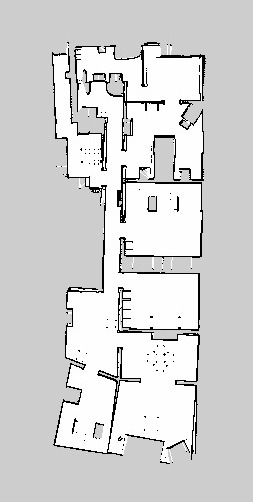
\includegraphics[width=0.4\textwidth, angle=90]{occ_map_img.jpg}
\end{center}
\caption{Ejemplo de mapa de ocupación}
\end{figure}

\section{Sensores RGBD}

Las cámaras RGBD son sensores visuales que, además de ofrecer información de color del entorno, proporcionan la distancia a la que se encuentra cada píxel de la imagen. Son cámaras a color comunes a las que se le añade un sensor de profundidad (normalmente, sensores infrarrojos) junto con un procesamiento que les permite percibir e interpretar la distancia a la que se sitúan los diferentes elementos del entorno que estén dentro de su campo de visión.\\

\addimage{kinect_img.png}{kinect}{Kinect V1}{0.5}

Algunos de los fabricantes más importantes de este tipo de sensores son Microsoft, con la conocida Kinect; ASUS, IFM, StereoLabs, Intel, Orbbec, etc.\\

\subsection{Imagen de profundidad}

La imagen de profundidad, al igual que cada uno de los canales de color RGB, es una matriz donde cada valor representa un nivel de gris asociado a una distancia y está referido a cada uno de los píxeles que componen la imagen. Las dimensiones de esta imagen vendrán determinadas por la resolución de la cámara, es decir, si por ejemplo la resolución de la cámara es de 640x480 píxeles, la matriz tendrá 480 filas y 640 columnas. \\

\addimage{depth_img.png}{depth}{Ejemplo de imagen de profundidad}{0.7}

El valor de distancia para cada píxel establece un nivel de gris. Generalmente, los objetos situados más alejados del sensor tendrán valores más claros, mientras que a los más cercanos se le asignan valores más oscuros. Esta información se decodifica para obtener así la información absoluta en distancia, típicamente en metros o milímetros, dependerá de la codificación con la que la cámara envía la información.\\

\section{Nubes de puntos}

Una nube de puntos o pointcloud es un conjunto de vértices en un sistema de coordenadas tridimensional. Estos vértices se identifican habitualmente como coordenadas X, Y y Z y son representaciones de la superficie externa de un objeto. Se crean a partir de escáneres láser tridimensionales o imágenes de profundidad.\\

Las nubes de puntos tienen infinidad de aplicaciones como la elaboración de modelos 3D en CAD de piezas fabricadas, la inspección de calidad en metrología y muchas otras en el ámbito de la visualización, animación, texturización y aplicaciones de personalización masiva.\\

\addimage{pointcloud-img.png}{pc}{Ejemplo de nube de puntos}{0.7}

\section{YOLO: You only look once}

You only look once (YOLO) es un sistema en tiempo real de detección de objetos basado en rede neuronales convolucionales y deep learning. Su principal característica y la que le distingue de otros modelos para la detección de objetos es que solo requiere visualizar una única vez la imagen (haciendo honores a su acrónimo). Esta propiedad le permite ser más rápido que los modelos competidores permitiendo la detección en tiempo real en vídeos de hasta 30 FPS. Según comentan sus creadores, es 1000 veces más rápido que R-CNN y 100 veces más rápido que Fast R-CNN. \\

\addimage{grafica_rendimiento_yolov3.png}{rend}{Comparación con otros modelos}{0.8}

En la figura \ref{fig:rend} se muestra una gŕafica de la comparación de YOLOv3 con respecto a otros modelos. El tiempo de inferencia es mucho menor que el de los otros modelos y la métrica COCO mAP-50 es bastante decente, sobre todo teniendo en cuenta el bajo tiempo de inferencia.\\

El procedimiento de YOLO es sencillo. Primero divide la imagen en una cuadrícula de $SxS$ y en cada una de estas celdas precide N posibles bounding boxes y calcula su probabilidad. Tras el cálculo, se eliminan aquellas que no superen un umbral de probabilidad. A las bounding boxes restantes, se les somete a un proceso de supresión de no máximos con el objetivo de eliminar los objetos que fueron detectados por duplicado, obteniéndose el resultado de la figura \ref{fig:proced}.\\

\addimage{yolo_proced.png}{proced}{Procedimiento de YOLO}{0.8}

YOLO es fácilmente implementable en ROS gracias al paquete darknet\_ros, que permite utilizarlo tanto en GPU como en CPU. La ventaja de usar la GPU para lanzar el modelo es que es 500 veces más rápido que utilizando la CPU. Para utilizar la GPU es necesario instalar el software CUDA de Nvidia.\\

(Fuente: \url{https://pjreddie.com/darknet/yolo/} además tiene un PAPER)\\

\subsection{Compute Unified Device Architecture}

CUDA es un conjunto de herramientas de desarrollo creadas por Nvidia que permiten a los programadores usar una variación del lenguaje de programación C (CUDA C) para coificar algoritmos GPU de Nvidia. Tiene como objetivo explitar las ventajas de las GPU frente a las CPU de propósito general utilizando el paralelismo que ofreccen sus múltiples núcleos, que permiten lanzar un altísimo número de procesos simultáneos.\\

Las principales ventajas de este sistema de computación son:

\begin{itemize}

	\item Lecturas dispersas. Se puede consultar cualquier posición en memoria.
	\item Memoria compartida. CUDA pone a disposición un área de memoria de entre 16KB y 48KB que se compartirá entre hilos del mismo bloque, pudiéndose utilizar como memoria caché.
	\item Lecturas más rápidas de y hacia la GPU.
	\item Soporte para enteros y operadores a nivel de bit.

\end{itemize}

Fuente: \url{https://es.wikipedia.org/wiki/CUDA}\\


\chapter{Diseño e implementación}

Para implementar el sistema que nos permita obtener estos mapas de ocupación a partir de la imagen de profundidad generada por una cámara RGB-D, se utilizarán una serie de nodos de ROS. Algunos de estos paquetes y nodos son proporcionados por la comunidad de usuarios de ROS. Otros son diseñados expresamente para este proyecto.\\

Primeramente se realizará una visión general de todo el conjunto de nodos y paquetes. Se explicará el camino que llevará la información y las formas que tienen los nodos de comunicarse.\\

Sobre los paquetes de terceros, se hará una breve explicación sobre la función que tienen de fábrica y la funcionalidad que se le han dado en este trabajo, así como el modo de comunicación con todo el árbol de nodos.\\

\section{Vista general del sistema}

Como se ha comentado, el objetivo es transformar la imagen de profundidad que se obtiene de un sensor RGBD en un láser artificial para generar un mapa de ocupación. En otro proceso, simultáneamente o de forma asíncrona, se generará un archivo TXT con los elementos detectado por YOLO de la imagen de color para tener un registro y poder analizarlo. En la figura X se muestra el árbol de nodos y topics de todo el sistema. Los nodos que han sido creados se muestran en color azul. Los nodos que han sido obtenidos de otras fuentes pero han necesitado de alguna modificación en su código se muestran en color naranja. Los nodos que hno se han modificado se muestran en blanco Los topics se representan con una caja de color blanco.\\

\addimage{esquema_general.png}{esq_general}{Árbol de nodos y topics}{1}

Primeramente, se obtiene la información del robot mediante la reproducción de un rosbag (más información en la sección \ref{sec:datos}). De este rosbag se obtienen mensajes en cuatro topics (entre otros): 

\begin{itemize}

	\item \texttt{/camera\_down/depth/image}. Imagen de profundidad de la cámara.
	\item \texttt{/tf}. Árbol de transformadas.
	\item \texttt{/amcl\_pose}. Pose del robot.
	\item \texttt{/camera\_down/rgb/image\_raw/compressed}. Imagen de color comprimida de la cámara.

\end{itemize}

El primero de los topics contiene mensajes de tipo \texttt{sensor\_msgs/Image} con información de la imagen de profundidad captada por la cámara. A partir de este mensaje generamos el mensaje de tipo \texttt{sensor\_msgs/CameraInfo} con información de la cámara mediante el nodo \texttt{cam\_info}. Luego se sincronizan estos dos mensajes con el nodo \texttt{sync\_info} y se envían por los topics \texttt{/sync/depth\_image} y \texttt{/sync/camera\_info}. Estos mensajes los recibe el nodo \texttt{depthimage\_to\_laserscan} y los procesa para generar el mensaje de tipo \texttt{sensor\_msgs/LaserScan} y enviarlos por el topic \texttt{/new\_scan}. Estos mensajes, juntos con los de tipo \texttt{tf2\_msgs/TFMessage} del topic \texttt{/tf}, los recibe el nodo \texttt{slam\_gmapping} y los transforma en un mapa o rejilla de ocupación que envía por el topic \texttt{/map} con el formato \texttt{nav\_msgs/OccupancyGrid}. \\

Con el topic \texttt{/camera\_down/rgb/image\_raw/compressed} se obtienen mensajes de tipo \texttt{sensor\_msgs/CompresedImage}. Con el nodo \texttt{republish} se descomprimen y se envían por el topic \texttt{/camera\_down/rgb/image\_raw/decompressed}. Estos mensajes los recibe la red neuronal mediante el nodo \texttt{darknet\_ros} y envía mensajes de tipo \texttt{darknet\_ros\_msgs/BoundingBoxes} por el topic \texttt{/darknet\_ros/bounding\_boxes}. El nodo \texttt{write\_objects} procesa estos mensajes y los de la pose del robot de tipo \texttt{sensor\_msgs/PoseWithCovarianceStamped} del topic \texttt{/amcl\_pose} y les da formato de tabla para pasarlos a un archivo TXT.\\


\section{Fuente de datos} \label{sec:datos}

La mejor manera de comprobar el correcto funcionamiento de todo el conjunto de nodos sería hacerlo directamente sobre el robot, con información real de sensores y del entorno. Sin embargo, debido a la dificultad que supondría utilizar este sistema sobre el robot, se decidió optar por otras vías.\\

Un  rosbag de ROS es una herramienta que permite capturar todos los mensajes que se publican por determinados topics para luego reproducirlos. Esto permite ejecutar el robot una única vez capturando todos los topics y luego reproducir los mensajes de estos topics cuantas veces queramos, permitiendo probar los nodos que se estén desarrollando sin tener que hacerlo directamente sobre el robot. Toda esta información se guarda en un archivo .bag.\\

Para este proyecto se va a utilizar un rosbag generado por uno de los robots del laboratorio de Automática de la Escuela Técnica Superior de Informática. Esta grabación recoge la información de la pose del robot (posición X e Y y el ángulo de orientación), los datos recogidos por una cámara RGB-D (color y profundidad), el barrido de un láser y otra información que típicamente se utiliza en los robots como el árbol de transformadas.\\

\subsection{Adaptación del rosbag}

Sin embargo, pese a que este rosbag ha sido el utilizado para comprobar el funcionamiento del algoritmo diseñado, ha sido necesario hacer algunas modificaciones para que se pueda procesar la información correctamente.\\

Normalmente, cuando se utiliza una cámara RGB-D en ROS, el paquete encargado de controlar la cámara envía tres tipos de mensajes pertenecientes al paquete sensor\_msgs. Estos mensajes son:

\begin{itemize}

	\item Imagen a color. Información de color de la imagen capturada con un mensaje de tipo Image. La mayoría de cámaras ofrece además la imagen rectificada, sin distorsiones.
	\item Imagen de profundidad. Información sobre la profundidad de la imagen capturada con un mensaje de tipo Image. Al igual que con la de color, también se ofrece la imagen rectificada.
	\item Parámetros de la cámara. Información sobre las propiedades de la cámara con un mensaje de tipo CameraInfo. Contiene datos sobre las propiedades de la imagen (ancho y alto) y parámetros de calibración de la cámara.

\end{itemize}

Debido a algunos problemas que se tuvieron durante la captura de los datos, este último topic no se ofrece en el rosbag, por lo que es necesario generarlo externo al rosbag. Para ello, se ha diseñado un nodo llamado cam\_info que se encarga de generar este mensaje que más tarde será utilizado por otros nodos.\\

\addimage{cam_info-diag.png}{cam_info}{Diagrama del nodo cam\_info}{1}

Este nodo, programado en C++, recibe el mensaje de la imagen de profundidad ofrecido por el rosbag, copia su encabezado, crea el mensaje de tipo CameraInfo con los parámetros de la cámara y lo envía por el topic /camera\_info. Estos parámetros han sido dados por la persona que generó el rosbag.[*Indicar los parámetros utilizados].\\

Finalmente, una vez generado el mensaje con la información de los parámetros de la cámara, es necesario sincronizar estos topics para que puedan ser utilizados por otros nodos. Para ello se ha diseñado un nodo en Python llamado sync\_info que se sirve del paquete message\_filter para realizar este proceso. Se ha programado en Python porque resulta más fácil utilizar esta librería en este lenguaje que en C++.\\

\addimage{sync_info-diag.png}{sync_info}{Diagrama del nodo sync\_info}{1}

Con la adición de estos nodos ya se tendría la información correcta para utilizar los otros paquetes sin ningún problema.\\

\subsection{Otras fuentes tomadas en cuenta}

Inicialmente, se propuso trabajar con un rosbag obtenido a partir de la ejecución de un robot virtual en un entorno simulado en Unity. Este entorno estaba ambientado en una vivienda común, con mobiliario típico y sin demasiados objetos en escena. Esto probablemente hubiera dado un mejor resultado que el rosbag que finalmente se utilizó ya que este último fue ejecutado en un laboratorio con muchos elementos que dificultan la labor del algoritmo (ventanas, entrantes y salientes, gran cantidad de objetos).\\

Sin embargo, la decodificación de la imagen de profundidad ocasionó muchos problemas que se escapaban del ámbito de este proyecto por lo que se decidió tomar otra vía.\\

\section{De imagen de profundidad a barrido láser}

Una vez se tiene toda la información ofrecida por el robot y la cámara correctamente sincronizada y configurada, es momento de realizar el procedimiento principal de este proyecto: transformar la imagen de profundidad obtenida mediante la cámara RGB-D en un barrido láser equivalente, cogiendo la distancias más alejadas captadas en la imagen. De esta forma, si tenemos varios objetos delante de una pared, con el algoritmo diseñado no se tendrán en cuenta estos objetos y se seleccionarán siempre las distancias menos restrictivas para generar el láser. Es necesario generar un láser artificial porque los algoritmos que se utilizan para generar el mapa de ocupación utilizan este tipo de datos.\\

El algoritmo utilizado está basado en el paquete de ROS depthimage\_to\_laserscan. Este paquete se encarga de transformar una imagen de profundidad en un barrido láser a partir de los parámetros de la cámara y de una serie de parámetros de entrada configurables. Estos parámetros son:

\begin{itemize}

	\item scan\_height. Establece la cantidad de filas que se quieren procesar para generar el láser. 
	\item scan\_time. Establece el tiempo de actualización entre escaneos. Por defecto está a 0.033 (30 FPS).
	\item range\_min. Rango de distancia mínima. Valores medidos menores que este valor se tomarán como -Inf. Por defecto está a 0.45 (metros).
	\item range\_max. Rango de distancia máxima. Valores medidos mayores que este valor se tomarán como +Inf. Por defecto está a 10 (metros).
	\item output\_frame\_id. Establece el id del eje de coordenadas (frame) de salida. Se indica el id del frame del láser.

\end{itemize}

[Añadir imagen de comparación del laser]

Este nodo primeramente recibe la imagen de profundidad y la información de la cámara. Se recuerda que estos mensajes los debe recibir a la vez y por eso requería de la sincronización. Una vez recibidos estos mensajes, evalúa la codificación de la imagen. Si la codificación es correcta (admite codificación 16UC1 o 32FC1[*Explicar los de los encodings]), procede a convertir la imagen de profundidad a un mensaje de tipo LaserScan.\\

Un mensaje de tipo LaserScan se forma a partir de las siguientes características:

\begin{itemize}

	\item header. Encabezado del mensaje. Propiedad que tienen todos los mensajes.
	\item angle\_min. Ángulo mínimo que abarca el láser en radianes.
	\item angle\_max. Ángulo máximo en radianes.
	\item angle\_increment. Ángulo entre medidas en radianes.
	\item time\_increment. Tiempo entre medidas en segundos.
	\item scan\_time. Tiempo entre escaneos en segundos.
	\item range\_min. Rango mínimo del sensor en metros.
	\item range\_max. rango máximo del sensor en metros.
	\item ranges. Vector con las medidas tomadas en metros.
	\item intensities. Vector con las intensidades de las medidas. Lo tomaremos como un array vacío porque no es necesario.

\end{itemize}

El algoritmo se encarga de analizar tantas filas como se establezcan en el parámetro scan\_height del nodo depthimage\_to\_laserscan y transformar la distancia dada por la imagen de profundidad en una distancia real al sensor. Una vez transformada, se compara con la distancia de las otras filas medidas en la misma columna y, si la distancia es mayor, se añade al vector ranges. Una vez completado el análisis de todas las filas de la imagen, se publica el mensaje generado de tipo \texttt{sensor\_msgs/LaserScan} en el topic \texttt{/new\_scan}.\\

\section{Generación del mapa de ocupación}

Una vez obtenido el láser artificial a partir de la imagen de profundidad, es momento de generar el mapa o rejilla de ocupación. Para este procedimiento se utilizará el paquete \texttt{gmapping}.\\

Este paquete ofrece un sistema de Localización y Mapeado Simultáneo o SLAM (del inglés, \textit{Simultaneous Location and Mapping}) a través de un nodo llamado \texttt{slam\_gmapping}. Este nodo recibe el láser artificial (por el topic \texttt{/new\_scan}) y el árbol de transformadas (por el topic \texttt{/tf}). Además tiene varios parámetros.\\

Al lanzar este nodo, es posible establecer multitud de parámetros que determinan el modo de operación. Entre otros, los parámetros que se tendrán en cuenta son:

\begin{itemize}

	\item \texttt{linearUpdate}. El nodo procesará un escaneo cada vez que se alcance la distancia lineal determinada por este parámetro. Su valor por defecto es $1.0$. El valor óptimo encontrado tras múltiples pruebas es $0.3$.
	\item \texttt{angularUpdate}. Determina el incremento de ángulo por el cuál el robot procesará otro escaneo. Su valor por defecto es $0.5$. El valor óptimo es $0.7$.
	\item \texttt{temporalUpdate}. Establece cada cuánto se procesa un nuevo escaneo. Su valor por defecto y óptimo es $3.0$.

\end{itemize}

Como se comenta en el listado de parámetros, tienen unos valores por defecto que se han ido modificando para obtener un mapa con más fiable. Esto se comentará más en profundidad en la sección de resultados.\\

\section{Detección de objetos}

Paralelamente, se ha diseñado un sistema capaz de interpretar la imagen a color proporcionada por el sensor RGBD para detectar los objetos y tener un registro de los mismos. Este sistema, en principio, se puede lanzar simultáneamente junto con el sistema de generación de mapas de ocupación, sin embargo, debido a la potencia necesaria para ejecutar la red neuronal por GPU, resulta tedioso e incluso problemático con algunos ordenadores. Es por ello que se ha diseñado para que pueda ser lanzado de forma asíncrona con respecto al otro sistema.\\

\subsection{Descompresión de la imagen de color}

En muchas ocasiones, los paquetes de ROS que sirven para utilizar determinadas marcas de sensores RGBD proporcionan las imágenes en un formato comprimido para ahorrar espacio. Con el rosbag que se ha utilizado como fuente de datos ocurre lo mismo, por lo que es necesario un proceso de descompresión.\\

Para este procedimiento, se ha utilizado un nodo llamado \texttt{republish} del paquete \texttt{image\_transport}. Este nodo se recibe un mensaje en formato \texttt{sensor\_msgs/\-Compressed\-Image} y lo convierte en un mensaje de tipo \texttt{sensor\_msgs/Image} para publicarlo.\\

\subsection{Ejecución de YOLO}

Una vez la imagen está descomprimida, ya puede ser recibida por la red neuronal. Este nodo recibe la imagen de color en formato \texttt{sensor\_msgs/Image} y publica en tres topics:

\begin{itemize}

	\item \texttt{object\_detector}. Mensaje de tipo \texttt{std\_msgs/Int8} que indica el número de objetos detectados.
	\item \texttt{bounding\_boxes}. Mensaje de tipo \texttt{darknet\_ros\_msgs/BoundingBoxes} que representa un array que proprociona información sobre la posición y el tamaño de los bounding boxes en píxeles.
	\item \texttt{detection\_image}. Mensaje de tipo \texttt{sensor\_msgs/Image} que ofrece las bounding boxes detectadas sobre la imagen a color que ha sido procesada.
	
\end{itemize}

Las bounding boxes son unas ``cajas'' que señalizan al elemento detectado. Un mensaje de tipo \texttt{darknet\_ros\_msgs/BoundingBoxes} es un array de elementos con formato \texttt{darknet\_ros\_msgs/BoundingBox}.\\

Además, este nodo ofrece una salida en la terminal indicando los frames por segundo (FPS) a los que se está ejecutando y un listado de los objetos encontrados junto con sus probabilidades. YOLO tiene un umbral de probabilidad establecido por defecto en $0.7$ para aceptar una detección como válida o no. \\

Cabe mencionar que para utilizar YOLO con CUDA correctamente ha sido necesario un largo y tedioso proceso de configuración que se explicará en el Anexo X.\\

\section{Procesamiento de los objetos detectados}

Como se ha comentado, de YOLO obtenemos un array de bounding boxes con información sobre la posición y el tamaño en píxeles. Para el desarrollo de este proyecto se ha visto conveniente procesar esa información para realizar un posterior estudio de los objetos que han sido detectados y analizar de la fiabilidad de la red neuronal así como la calidad de los datos proporcionado por el rosbag.\\

Para este procesamiento se ha diseñado un nodo llamado \texttt{write\_objects} que se encarga de recibir los mensajes que se publican en \texttt{/darknet\_ros/bounding\_boxes} y en \texttt{/amcl\_pose} para generar un archivo CSV donde cada fila representa la información con el formato mostrado en el cuadro \ref{tab:formato}. Cada columna utilizará el delimitador de punto y coma (`` ; '').\\

\begin{table}[H]
\begin{center}
\begin{tabular}{| c | c | c | c | c |}
	\hline
	Objetos & Probs & Posición & Orientación & Tiempo \\ \hline
	obj1:obj2:...:objN & prob1:prob2:...:probN & pX:pY:pZ & oW:oX:oY:oZ & (seg) \\ \hline

\end{tabular}
\caption{Formato del archivo CSV generado}
\label{tab:formato}
\end{center}
\end{table} 

Toda esta información es obtenida a partir del formato de los mensajes de las bounding boxes y de la pose. Para las bounding boxes es necesario acceder a cada una de ellas y obtener sus propiedades \texttt{Class} y \texttt{probability}. Para la pose es necesario acceder a su propiedades \texttt{pose.pose.position} y \texttt{pose.pose.orientation}.\\

El formato del mensaje de una bounding box tiene las siguientes propiedades:

\begin{itemize}

	\item \texttt{probability}. Probabilidad de que el elemento detectado sea realmente de la clase que se le atribuye.
	\item \texttt{xmin}. Coordenada X mínima de la bounding box en píxeles.
	\item \texttt{ymin}. Coordenada Y mínima de la bounding box en píxeles.
	\item \texttt{xmax}. Coordenada X máxima de la bounding box en píxeles.
	\item \texttt{ymax}. Coordenada Y máxima de la bounding box en píxeles.
	\item \texttt{id}. Identificador único para cada bounding box.
	\item \texttt{Class}. Clase o etiqueta del elemento detectado.

\end{itemize}

Para la generación del archivo CSV se ha hecho uso de la librería 


\printbibliography

\end{document}